% XeLaTeX document for پاسخ تمرین اول مبحث فازی
\documentclass[12pt,a4paper]{article}
\usepackage{fontspec}
\usepackage{xepersian}
\settextfont{XB Niloofar}
\setlatintextfont{Times New Roman}
\usepackage{geometry}
\geometry{top=1.5cm, bottom=2cm, left=2cm, right=2cm}
\usepackage{xcolor}
\usepackage{float}
\usepackage{graphicx}
\usepackage{placeins}
\usepackage{hyperref}
\usepackage{amsmath}
\hypersetup{
	colorlinks=true,
	urlcolor=blue,
}
\usepackage{enumitem}
\setlist[itemize]{noitemsep, topsep=0pt}
\usepackage{titlesec}
\titleformat{\section}{\large\bfseries}{\thesection}{1em}{}

\begin{document}
	\begin{center}
		{\LARGE\textbf{پاسخ تمرین اول مبحث فازی}}\\[0.5em]
	\end{center}
	
	\section*{سؤال ۱: مجموعه فازی و تابع عضویت}
	مجموعهٔ فازی \lr{(Fuzzy Set)} مجموعه‌ای است که به هر عنصر \(x\in X\) یک درجه عضویت \(\mu_A(x)\in[0,1]\) نسبت می‌دهد. تابع عضویت \(\mu_A: X\to[0,1]\) نشان‌دهنده میزان تعلق عنصر به مجموعهٔ فازی است: مقدار صفر به معنی عدم تعلق و مقدار یک به معنی تعلق کامل.
	
	\section*{سؤال ۲: امکان همزمان درست و نادرست بودن}
	در منطق کلاسیک، یک گزاره یا درست (۱) است یا نادرست (۰). اما در منطق فازی می‌توان برای گزاره‌ها درجاتی بین صفر و یک اختصاص داد؛ بنابراین یک گزاره می‌تواند تا حدودی درست و تا حدودی نادرست باشد که این انعطاف در مدل‌سازی واقعیت انسانی مفید است.
	
	\section*{سؤال ۳: تشخیص مجموعه فازی از مجموعه قطعی}
	اگر تابع عضویت مجموعهٔ \(A\) تنها مقادیر ۰ و ۱ بگیرد، آن مجموعه قطعی است. اما اگر
	\[
	\exists x:\ \mu_A(x)\in(0,1)
	\]
	آنگاه مجموعه فازی است، زیرا درجه‌ای از تعلق بین صفر و یک وجود دارد.
	
	\section*{سؤال ۴: فازی‌سازی متغیرهای واقعی}
	\begin{itemize}
		\item درآمد (پوند): متغیرهای فازی «درآمد کم»، «متوسط»، «زیاد» — برای تعیین مرز دقیق دشوار.
		\item سرعت (متر بر ثانیه): «سرعت کم»، «متوسط»، «زیاد» — مرزها پیوسته‌اند.
		\item علاقه به تماشای تلویزیون: «خیلی کم»، «کم»، «متوسط»، «زیاد»، «خیلی زیاد» — ذهنی است.
		\item تمایل به خوردن وعده غذایی: «اصلاً ندارم»، «کم»، «متوسط»، «زیاد»، «خیلی زیاد» — پیوسته و ذهنی.
		\item رنگ چراغ راهنمایی: \textbf{نیاز نیست} — رنگ‌ها از پیش تعریف‌شده و قطعی‌اند.
	\end{itemize}
	متغیر «رنگ چراغ راهنمایی» فازی‌سازی نمی‌شود چون حالت‌ها قطعی و محدود هستند.
	
	\section*{سؤال ۵: سیستم خبره فازی پیش‌بینی وضعیت هوا}
	\begin{enumerate}[label=\alph*)]
		\item برای فشار هوا \(P=1020\,\mathrm{mbar}\):
		\[
		\mu_{\mathrm{پایین}}\approx0,\quad
		\mu_{\mathrm{وسط}}\approx0.6,\quad
		\mu_{\mathrm{بالا}}\approx0.2
		\]
		\FloatBarrier 
		\begin{figure}[H]
			\centering
			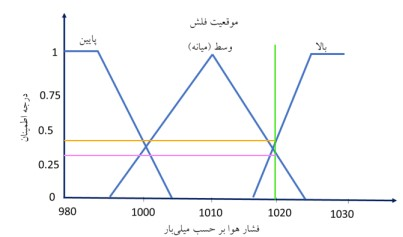
\includegraphics[width=0.7\textwidth]{5a.jpg}
			\caption*{شکل ۵-الف: توزیع تابع عضویت برای فشار \(P=1020\,\mathrm{mbar}\)}
		\end{figure}
		\item برای نرخ تغییر فشار \(\dot P=-2\,\mathrm{mbar/h}\):
		\[
		\mu_{\mathrm{به\ پایین}}\approx0.7,\quad
		\mu_{\mathrm{ثابت}}\approx0.3
		\]
		\FloatBarrier 
		\begin{figure}[H]
			\centering
			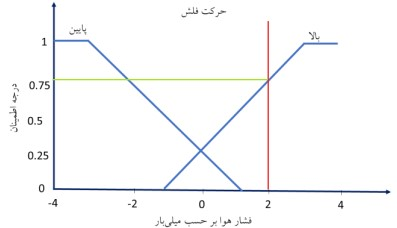
\includegraphics[width=0.7\textwidth]{5b.jpg}
			\caption*{شکل ۵-ب: توزیع تابع عضویت برای نرخ تغییر فشار \(\dot P=-2\,\mathrm{mbar/h}\)}
		\end{figure}
		\item با ترکیب درجات عضویت در شروط و ضریب اطمینان قواعد:
		\[
		\text{حجم نفوذ هر قاعده} = \min\bigl(\mu_{\text{شرط1}},\mu_{\text{شرط2}}\bigr)\times\text{اعتماد}
		\]
		سپس برای نتیجه «ابری» درجه نهایی برابر با
		\[
		\max\{\text{نفوذ قواعد منتهی به ابری}\}
		\]
	\end{enumerate}
	
	\section*{سؤال ۶: نقاط قوت و ضعف سیستم‌های فازی نسبت به سیستم‌های قطعی}
	\subsection*{نقاط قوت}
	\begin{itemize}
		\item \textbf{مدل‌سازی عدم قطعیت و نادقیق بودن اطلاعات:} داده‌های واقعی معمولاً مبهم و ناقص‌اند و سیستم‌های فازی می‌توانند با آن‌ها بهتر کار کنند.
		\item \textbf{تفسیرپذیری و شباهت به منطق انسانی:} قواعد ساده و به زبان طبیعی نوشته می‌شوند و خروجی سیستم برای انسان قابل فهم‌تر است.
		\item \textbf{عدم نیاز به مدل دقیق ریاضی:} نیاز نیست مدل صریح ریاضی مسئله استخراج شود؛ می‌توان از دانش کارشناسان بهره برد.
	\end{itemize}
	
	\subsection*{نقاط ضعف}
	\begin{itemize}
		\item \textbf{تنظیم تجربی پارامترها:} انتخاب توابع عضویت و مقادیر آن‌ها غالباً سلیقه‌ای است و نیاز به آزمون و خطا دارد.
		\item \textbf{افزایش پیچیدگی با بزرگ شدن مسئله:} تعداد قواعد با افزایش ورودی‌ها زیاد می‌شود و مدیریت سیستم دشوار می‌گردد.
		\item \textbf{وابستگی به دانش انسانی:} کیفیت سیستم به دانش و تجربهٔ کارشناسان اولیه بستگی دارد؛ خطا یا ناقص بودن دانش منجر به عملکرد ضعیف خواهد شد.
	\end{itemize}
	
	\section*{سؤال ۷: تفاوت Mamdani و TSK}
	در روش Mamdani خروجی هر قاعده یک مجموعه فازی است که پس از استنتاج و تجمع، با روش \lr{Defuzzification} به عدد می‌رسد. اما در روش TSK خروجی هر قاعده تابعی جبری (معمولاً خطی) از ورودی‌هاست و در انتها با میانگین‌گیری وزنی ترکیب می‌شود.
	
	\section*{سؤال ۸: TSK معمولی vs Piecewise Linear Fit}
	\begin{itemize}
		\item در TSK کلاسیک، توابع خروجی قواعد از پیش تعریف‌شده و اغلب خطی‌اند.
		\item در \lr{Piecewise Linear Fit} با یادگیری‌محور بخش‌های ورودی به قطعات تقسیم و توابع خطی در هر بخش یاد گرفته می‌شوند تا تقریب دقیق‌تر گردد.
	\end{itemize}
	
	\section*{سؤال ۹: رفع تضاد در سیستم‌های مبتنی بر دانش}
	روش‌های معمول:
	\begin{itemize}
		\item اولویت‌بندی قواعد
		\item انتخاب قاعده با بیشترین درجه مطابقت
		\item استراتژی تصادفی وزن‌دار
	\end{itemize}
	در سیستم فازی نیز با اپراتورهای \lr{min} و \lr{max} و تجمیع خروجی‌ها تضاد برطرف می‌شود.
	
	\section*{سؤال ۱۰: یادگیری پارامترهای TSK}
	پارامترهای توابع عضویت و ضرایب توابع خروجی با استفاده از الگوریتم‌های بهینه‌سازی مانند \lr{Gradient Descent} یا روش‌های ژنتیکی تنظیم می‌شوند تا خطای سیستم روی داده‌های آموزشی کمینه شود.
	
\end{document}